



%----------------------------------------------------------------------------------------

\newpage

%%%%%%%%%%%%%%%%%%%%%%%
\section{Static Correlations}{Correlations Statiques}

\label{app:sec:staticcorrelations}



%%%%%%%%%%%%%%%%%%%%%%%
\subsection{Morphological Measures}{Mesures morphologiques}



% No need fo distributions, maps enough.
%%%%%%%%%%%%%%%%%%%
%\begin{figure}
%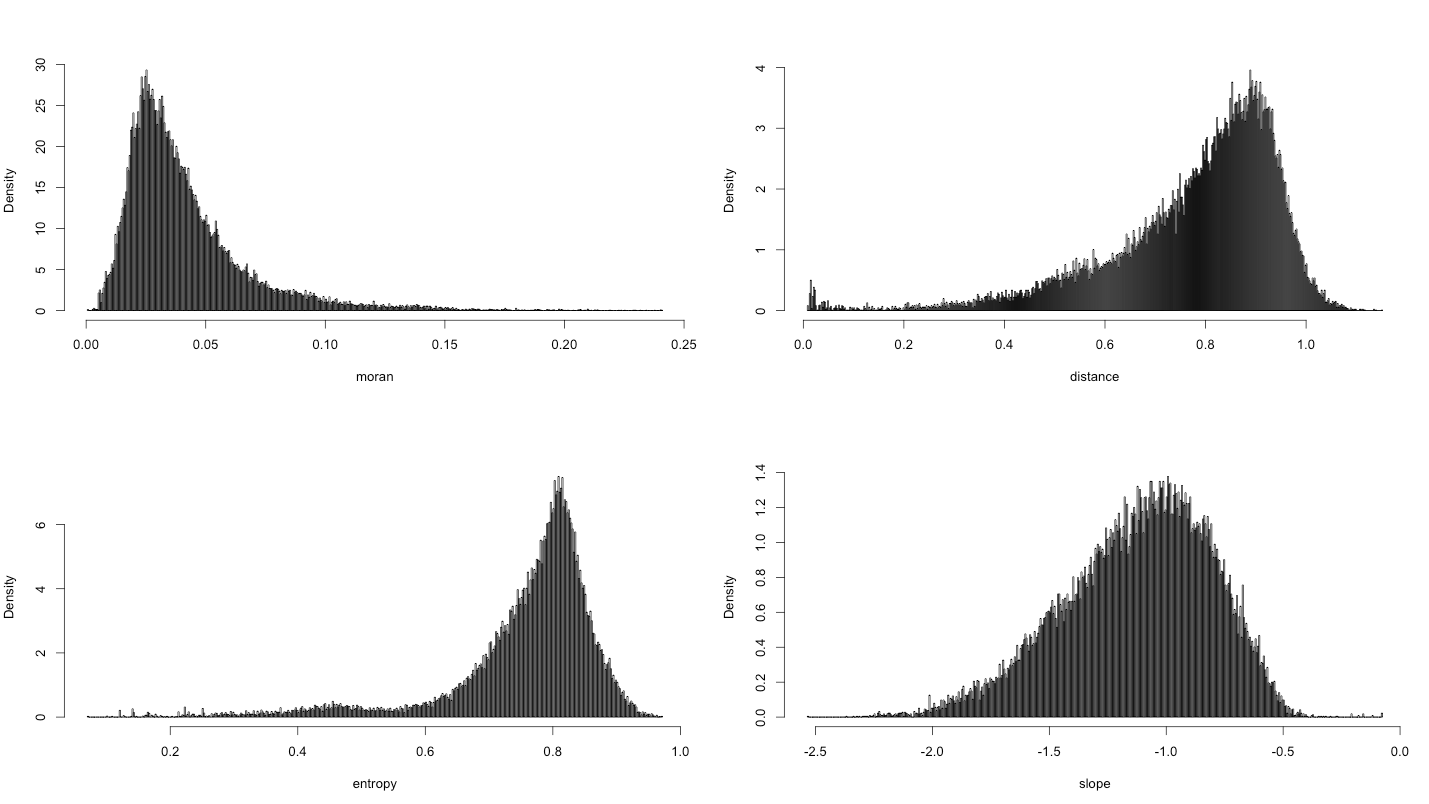
\includegraphics[width=1.2\textwidth]{Figures/Static/Density/hists_GOOD}
%\caption[Empirical Distribution of Morphological Indicators]{Empirical Distribution of Morphological Indicators}{Distribution empirique des indicateurs morphologiques\comment{(Florent) titres/labels illisibles ; dans quelle perspective as tu calculé ces indicateurs/affiché l'histogramme ?}}
%\end{figure}
%%%%%%%%%%%%%%%%%%
%



%%%%%%%%%%%%%%%%%%%%%%%
\subsection{Network Simplification Algorithm}{Algorithme de Simplification du Réseau}

% data collected from http://download.geofabrik.de/europe.html : bosse pas sur le fichier world, huge.

 
 
More precisely we use the following procedure :
\begin{itemize}
\item a background raster (which resolution $r$ gives the snapping parameter for aggregation) is constructed from a reference raster and the extent of network. This grid gives spatial aggregation units for network nodes.
\item for each feature of the road dataset, corresponding connected raster cells are stored with corresponding impedance and distance in a sparse adjacency matrix.
\item Network is simplified by iterative suppression of nodes with degree two, with keeping link speed and real length to their effective value.
\end{itemize}

% \cite{2016arXiv161101890B} : interactive appli for network simplification



\paragraph{Implementation}{Implémentation}

A \texttt{PostGIS} database is used to store raw and simplified network, in order to perform efficient spatial requests, compared for example to initial \texttt{osm} data formats (\texttt{osm} or \texttt{pbf}). However the size of storage of data into this base is much higher (factor 10) so processing was parallelized between european countries. Consistence is ensured by the use of the same common density raster as simplification canvas. Final network is stored into the Postgis database for efficient indicator computation given a spatial extent. \comment{(Florent) y'a t'il un effet de bord dans les carrés 50x50 qui se trouvent à la frontière de 2 pays}[pas avec nouvelle parallelisation pas par pays mais par split and merge (TODO rewrite nouvel algo)]


\paragraph{Sensitivity to simplification parameters}{Sensibilité aux paramètres de simplification}

Sensitivity of indicators to raster resolution and to degree simplification algorithm must still be tested to ensure the relevance of data preprocessing.



% example of simpl stage
 %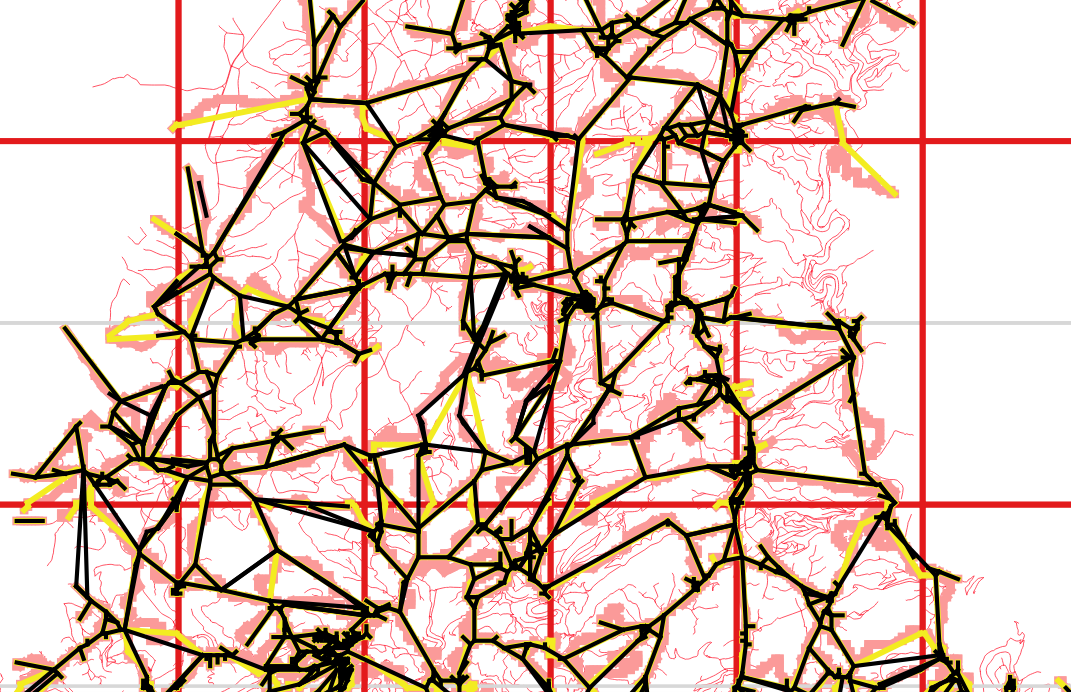
\includegraphics[width=\textwidth,height=0.5\textheight]{figures/ex_nw}






%%%%%%%%%%%%%%%%%%%%%%%
\subsection{Network Resilience}{Résilience des Réseaux}





La description complète d'un réseau suppose la donnée d'une grande quantité d'information, puisque la moitié de la matrice d'adjacence est nécessaire dans le cas non-dirigé (matrice complète dans le cas dirigé). L'établissement de typologies, c'est à dire de sortes de classes d'équivalence topologiques au sens large, est une façon de voir les enjeux de la recherche actuelle sur les réseaux : existe-t-il des formes typiques de réseau, et comment les représenter dans une dimension réduite ? Relativement importante est la dimension épistémologique de cette interrogation fondamentale, qui peut sous certaines hypothèses être ramenée à l'opposition d'un réductionisme à une vision intrinsèque de la complexité. Si une classification systématique réductrice existe pour tout système complexe, alors les niveaux d'émergence supérieurs n'ont pas de signification propre. Il est paradoxal d'observer dans ce cas la position ambigüe de certains travaux de physiciens qui tiennent ce réductionisme comme un dogmatisme mais prétendent s'attaquer à des problèmes complexes typiques des systèmes socio-techniques.

Les mesures de réseau globales comme nous avons vu en cours sont une façon de répondre partiellement à cette question de réduction dimensionnelle. En pratique, on veut être également capable de relier ces mesures à des propriétés pratiques du réseau, qui seront cruciales pour le design et le management de réseaux réels (par exemple réseaux techniques : transport d'électricité, internet ; réseaux de transport ; réseaux sociaux ; réseaux de villes ; etc.) : par exemple le coût, la résilience, la performance. Cet exercice propose de survoler ces deux questions fondamentales pour différents exemples de réseaux réels et synthétiques : illustrer dans un premier temps la signification concrète de différentes valeurs en relation à la topologie ``apparente'' du réseau ; dans un second temps explorer des liens potentiels entre mesures et propriétés afin de donner une idée d'une manière de caractériser la résilience.

Ce qui est demandé pourra paraître relativement simple mais est central pour une appréhension juste de la complexité des processus géographiques tels qu'ils occurrent dans toute leur réalité. La table~\ref{tab:measures} donne les valeurs d'indicateurs, pour certains types de réseaux. On fournit leur valeur moyenne et leur écart-type dans le cas de réseaux synthétiques aléatoires pour lesquels les mesures auront alors été estimées sur $b=500000$ répétitions des réseaux aléatoires.\footnote{qu'on fixe comme arbitraire. Le problème du nombre de répétitions nécessaires pour une convergence raisonnable des indicateurs statistiques et hors du champ de ce devoir, et d'ailleurs un problème ouvert pour la plupart des modèles de simulation complexes puisque qu'on sait établir des intervalles de confiances soit sous certaines hypothèses théoriques de distribution statistique soit par simulation (\emph{bootstrap}) ce qui ne réduit pas la complexité intrinsèque.} Pour les réseaux réels ou synthétiques non variables, une valeur seule est donnée, sachant que l'estimation de paramètres moyens dans des situations réelles est directement liée à la stationnarité spatio-temporelle des processus\footnote{et donc à leur ergodicité, i.e. à l'équivalence entre moyenne spatiale et moyenne temporelle}, ce qui est également une question ouverte concernant les systèmes spatiaux complexes. Les figures~\ref{fig:examples} et ~\ref{fig:real} illustre des exemples des réseaux considérés. Les questions suivantes portent sur une interprétation simple des mesures. Parmi les réseaux considérés, on étudie des réseaux routiers réels, dont la localisation spatiales est présentée en figure~\ref{fig:loc}, ainsi que des réseaux synthétiques.

Les réseaux étudiés sont donc les suivants\footnote{chaque générateur synthétique a des paramètres propres, pour lesquels nous choisissons les valeurs par défaut suivantes : probabilité aléatoire d'Erdos-Renyi $p=0.005$ ; proportion de liens de la grille conservés $65\%$ ; attachement préférentiel : nouveau liens $m=10$, exposant $\alpha=1$, exposant de vieillissement $\beta = -2$, pas de vieillissement 100 ; nombre de feuille par branche de l'arbre $f=3$.} : 
\begin{itemize}
\item Réseau routiers réels (simplifiés à une résolution de 100m) : Paris, Ile-de-France, La Courtine (Creuse), Grand Lyon, London Metropolitan Area, Randstad
\item Aléatoire (probabilité fixe d'établir un lien entre chaque paire de noeud)
\item Attachement préférentiel (type Barabasi-Albert : les liens sont établis itérativement avec une probabilité proportionnelle au degré des noeuds)
\item Grille perturbée (grille régulière dont on retire une proportion fixée de liens)
\item Arbre (au nombre de feuilles par branche fixe)
\end{itemize}

Les mesures calculées pour un réseau $N=(V,E)$ sont :

\begin{itemize}
\item Statistiques descriptives : nombre de noeuds $\left|V\right|$ et nombre de liens $\left|E\right|$
\item Densité $\gamma$
\item Degré moyen $\bar{d}$
\item Diamètre\footnote{pour toutes les mesures liées au plus courts chemins, les distances topologiques et non pondérées ont été prises en compte, afin de permettre la comparabilité des réseaux réels et des réseaux synthétiques. Pour une comparabilité des réseaux réels ayant des couvertures géographiques d'étendue significativement différentes, il faut normaliser par le diamètre.} $\delta$
\item Centralité d'intermédiarité $b$ : s'agissant d'une mesure locale (associée ici aux liens), on considère sa moyenne $<b>$ et son niveau de hiérarchie\footnote{donné par la pente de la regression linéaire d'un fit brutal d'une loi rang-taille : $\log{b_i} = \beta + \alpha\cdot \log i$ où les $b_i$ sont triés par ordre decroissants.} $\alpha\left[b\right]$
\item Centralité de proximité $c$ : de même on calcule $<c>$ et $\alpha\left[c\right]$
\item Efficacité $e = \frac{2}{n\cdot (n-1)} \sum_{i<j} \frac{1}{d_{ij}}$ avec $d_{ij}$ distance topologique entre $i$ et $j$
\item Coefficient de clustering $t$, qui donne la probabilité que les voisins d'un noeud soient connectés
\item Modularité $\mu$ qui donne une mesure plus générale de la structure en communauté du graphe
\end{itemize}



%%%%%%%%%%%%%%
\begin{table}
\hspace{-1cm}
\begin{tabular}{c|c|c|c|c|c|c|c|c|c|c|c|c}
\hline
Réseau & $\left|V\right|$ & $\left|E\right|$ & $\gamma$ & $\bar{d}$ & $\delta$ & $<b>$ \\\hline
Aléatoire & $1000$ & $2498 \pm 50 $ & $0.005 \pm 1\cdot 10^{-4} $ & $5 \pm 0.1 $ & $9 \pm 0.59 $ & $0.0018 \pm 5.4\cdot 10^{-5} $\\\hline
Att. Préf. & $1000$ & $4579 \pm 21 $ & $0.0092 \pm 4.3\cdot 10^{-5} $ & $9.2 \pm 0.043 $ & $7 \pm 0.18 $ & $0.00084 \pm 8.6\cdot 10^{-6} $\\\hline
Grille & $499\pm 3.7 $ & $624$ & $0.005 \pm 7.5\cdot 10^{-5} $ & $2.5 \pm 0.019 $ & $53 \pm 4.5 $ & $0.03 \pm 0.0027 $\\\hline
Arbre & $1000$ & $999$ & $0.002$ & $2$ & $12$ & $0.0099$\\\hline
Ile-de-France & $\left|V\right|$ & $\left|E\right|$ & $\gamma$ & $\bar{d}$ & $\delta$ & $<b>$\\\hline
Paris & $\left|V\right|$ & $\left|E\right|$ & $\gamma$ & $\bar{d}$ & $\delta$ & $<b>$\\\hline
Grand Lyon & $\left|V\right|$ & $\left|E\right|$ & $\gamma$ & $\bar{d}$ & $\delta$ & $<b>$\\\hline
La Courtine & $\left|V\right|$ & $\left|E\right|$ & $\gamma$ & $\bar{d}$ & $\delta$ & $<b>$\\\hline
Randstad & $\left|V\right|$ & $\left|E\right|$ & $\gamma$ & $\bar{d}$ & $\delta$ & $<b>$\\\hline
London& $\left|V\right|$ & $\left|E\right|$ & $\gamma$ & $\bar{d}$ & $\delta$ & $<b>$\\\hline
\end{tabular}
\bigskip
\hspace{-1cm}
\begin{tabular}{c|c|c|c|c|c|c}
\hline
Réseau & $\alpha \left[b\right]$ & $<c>$ & $\alpha\left[c\right]$ & $e$ & $t$ & $\mu$\\\hline
Aléatoire & $-0.29 \pm 0.0092 $ & $0.46 \pm 0.68 $ & $-0.076 \pm 0.032 $ & $0.24 \pm 0.003 $ & $0.005 \pm 0.0011 $ & $0.45 \pm 0.0072 $\\\hline
Att. Préf. & $-0.63 \pm 0.015 $ & $0.26 \pm 0.0021 $ & $-0.062 \pm 0.0022 $ & $0.28 \pm 0.0018 $ & $0.079 \pm 0.0028 $ & $0.66 \pm 0.0082 $\\\hline
Grille & $-1.2 \pm 0.077 $ & $7.3 \pm 3.5 $ & $-0.99 \pm 0.31 $ & $0.072 \pm 0.0032 $ & $0$ & $0.87 \pm 0.0058 $\\\hline
Arbre & $-1$ & $0.1$ & $-0.094$ & $0.11$ & $0$ & $0.93$
\end{tabular}

\caption[][]{}{Valeurs de mesures de réseaux pour différents exemples typiques réels et synthétiques \label{tab:measures}}
\end{table}
%%%%%%%%%%%%%%



\bigskip


\paragraph{}{Formes Urbaines et indicateurs de réseaux}

Commentez qualitativement les différentes formes des systèmes territoriaux observées. On pourra par exemple se poser la question de la polycentricité d'une Méga-région Urbaine. Reliez ces observations aux valeurs prises par les indicateurs que vous jugez pertinents.


\medskip


\paragraph{}{Interprétation des Indicateurs}

Pour les réseaux synthétiques, commentez les valeurs prises par les indicateurs. Lesquelles étaient intuitivement attendues ? Dans quelle mesure est-on capable de caractériser et discriminer chaque type de réseau. De quel réseau synthétique s'attend-on à ce que les réseaux réels soient les plus proches ? Peut-on le confirmer par les indicateurs ?


\bigskip


Nous proposons à présent de tenter une caractérisation de la résilience des réseau. La définition utilisée prend en compte la capacité du réseau à rester performant face à la rupture de lien, comme proposé par~\cite{ash2007optimizing}. On considère la rupture aléatoire d'une proportion fixée $\alpha$ de liens, et on note $N_{\alpha}$ le réseau résultant de la suppression à partir du réseau $N$. L'indicateur de résilience au niveau $\alpha$ est alors défini par $r = \mathbb{E} \left[\Delta_{\alpha} e \right] = \mathbb{E}\left[ e\left(N_{\alpha}\right) - e\left(N\right)\right]$. On peut définir de même les variations des autres indicateurs. La structure de covariance des différentes variations, et en particulier la correlation avec la résilience, est un moyen indirect de caractériser la résilience, au sens de quel type de propriété permet au réseau d'augmenter sa résilience. La table~\ref{tab:corr} donne pour chaque réseau aléatoire les correlations estimées $\rho\left[X\right] = \hat{\rho}\left[\Delta_{\alpha} e,\Delta_{\alpha} X\right]$ où l'estimateur $\hat{\rho}$ est calculé en pratique sur une plage de valeurs pour $\alpha$ (de 0.5 à 0.95 par 0.05) et sur un nombre de répétitions fixé ($b=$, en faisant l'hypothèse que répéter sur le réseau est équivalent à répéter sur la suppression des liens).


%%%%%%%%%%%%%%
\begin{table}
\begin{tabular}{c|c|c|c|c|c|c|c|c|c|c|c|c}
\hline
Réseau & $\left|V\right|$ & $\left|E\right|$ & $\gamma$ & $\bar{d}$ & $\delta$ & $<b>$ & $\alpha \left[b\right]$ & $<c>$ & $\alpha\left[c\right]$ & $e$ & $t$ & $\mu$\\\hline
Aléatoire & $\left|V\right|$ & $\left|E\right|$ & $\gamma$ & $\bar{d}$ & $\delta$ & $<b>$ & $\alpha \left[b\right]$ & $<c>$ & $\alpha\left[c\right]$ & $e$ & $t$ & $\mu$\\\hline
Attachement Préférentiel & $\left|V\right|$ & $\left|E\right|$ & $\gamma$ & $\bar{d}$ & $\delta$ & $<b>$ & $\alpha \left[b\right]$ & $<c>$ & $\alpha\left[c\right]$ & $e$ & $t$ & $\mu$\\\hline
Grille Perturbée & $\left|V\right|$ & $\left|E\right|$ & $\gamma$ & $\bar{d}$ & $\delta$ & $<b>$ & $\alpha \left[b\right]$ & $<c>$ & $\alpha\left[c\right]$ & $e$ & $t$ & $\mu$\\\hline
\end{tabular}
\caption[][]{}{Correlations estimées \label{tab:corr}}
\end{table}
%%%%%%%%%%%%%%


\medskip

\paragraph{}{Caractérisation de la résilience}

Commentez à partir de la table des corrélations, pour les différents types de réseau, les facteurs influençant la résilience. Quel enseignement peut-on en tirer pour la conception de réseaux techniques par exemple ?



\paragraph{}{Résilience Dynamique et Topologie}

Les approches à la notion de résilience sont diverses et complémentaires. L'aspect dynamique, au sens par exemple du temps nécessaire au système pour retrouver son état initial après perturbation, est particulièrement intéressant pour les systèmes urbains. Dans le cas de réseaux où les noeuds ont leur dynamique propre, les solutions pour une définition robuste et universelle sont très récentes, comme celle proposée par~\cite{gao2016universal}.


Vous semble-t-il simple, dans le cas de dynamiques couplées au sein d'un réseau, d'isoler la contribution de la topologie du réseau de celle des dynamiques propres à la dynamique générale ? Dans quelle mesure serait-il alors complexe de quantifier la résilience dynamique dans une dimension réduite ?







%%%%%%%%%%%%%%
%\begin{figure}
%\centering
%\includegraphics[width=0.45\textwidth,height=0.3\textheight]{figures/random_lowres.png}
%\includegraphics[width=0.45\textwidth,height=0.3\textheight]{figures/lattice.png}\\
%\includegraphics[width=0.45\textwidth,height=0.3\textheight]{figures/pa-age_lowres.png}
%\includegraphics[width=0.45\textwidth,height=0.3\textheight]{figures/tree_lowres.png}
%\appcaption{Synthetic Networks}{Représentation d'instances des exemples synthétiques de réseaux. Dans l'ordre de haut en bas et de droite à gauche : réseau aléatoire, grille perturbée, attachement préférentiel, arbre.\label{fig:examples}}
%\end{figure}
%%%%%%%%%%%%%%

%%%%%%%%%%%%%%
%\begin{figure}
%\includegraphics[width=0.45\textwidth,height=0.3\textheight]{figures/idf_lowres.png}
%\includegraphics[width=0.45\textwidth,height=0.3\textheight]{figures/paris_lowres.png}\\
%\includegraphics[width=0.45\textwidth,height=0.3\textheight]{figures/lyon_lowres.png}
%\includegraphics[width=0.45\textwidth,height=0.3\textheight]{figures/lacourtine_lowres.png}\\
%\includegraphics[width=0.45\textwidth,height=0.3\textheight]{figures/randstad_lowres.png}
%\includegraphics[width=0.45\textwidth,height=0.3\textheight]{figures/londonM25_lowres.png}\\
%\appcaption{Real networks}{Réseaux routiers réels étudiés. Dans l'ordre de haut en bas et de droite à gauche : Ile-de-France, Paris, Grand Lyon, La Courtine, Randstad, London Metropolitan Area\label{fig:real}}
%\end{figure}
%%%%%%%%%%%%%%

%%%%%%%%%%%%%%
%\begin{figure}
%\centering
%\includegraphics[width=0.8\textwidth]{figures/areas}
%\appcaption{Localisation of networks}{Localisation Géographique des réseaux réels étudiés.}
%\label{fig:loc}
%\end{figure}
%%%%%%%%%%%%%%


% questions :
% - commentaires sur mesures ?
% - intuitivement, le plus sensible aux perturbations ?
% - matrice des correlations pour chaque type : lecture ; interpretation
% - comment mesurer correlations sur réseaux réels ?
% - vers une mesure dynamique de la résilience : question conceptuelle sur séparation dynamique/topologie - évoquer papier barabasi ?







\subsection{Network Indicators}{Indicateurs de réseau}


%%%%%%%%%%%%%%
\begin{figure}
%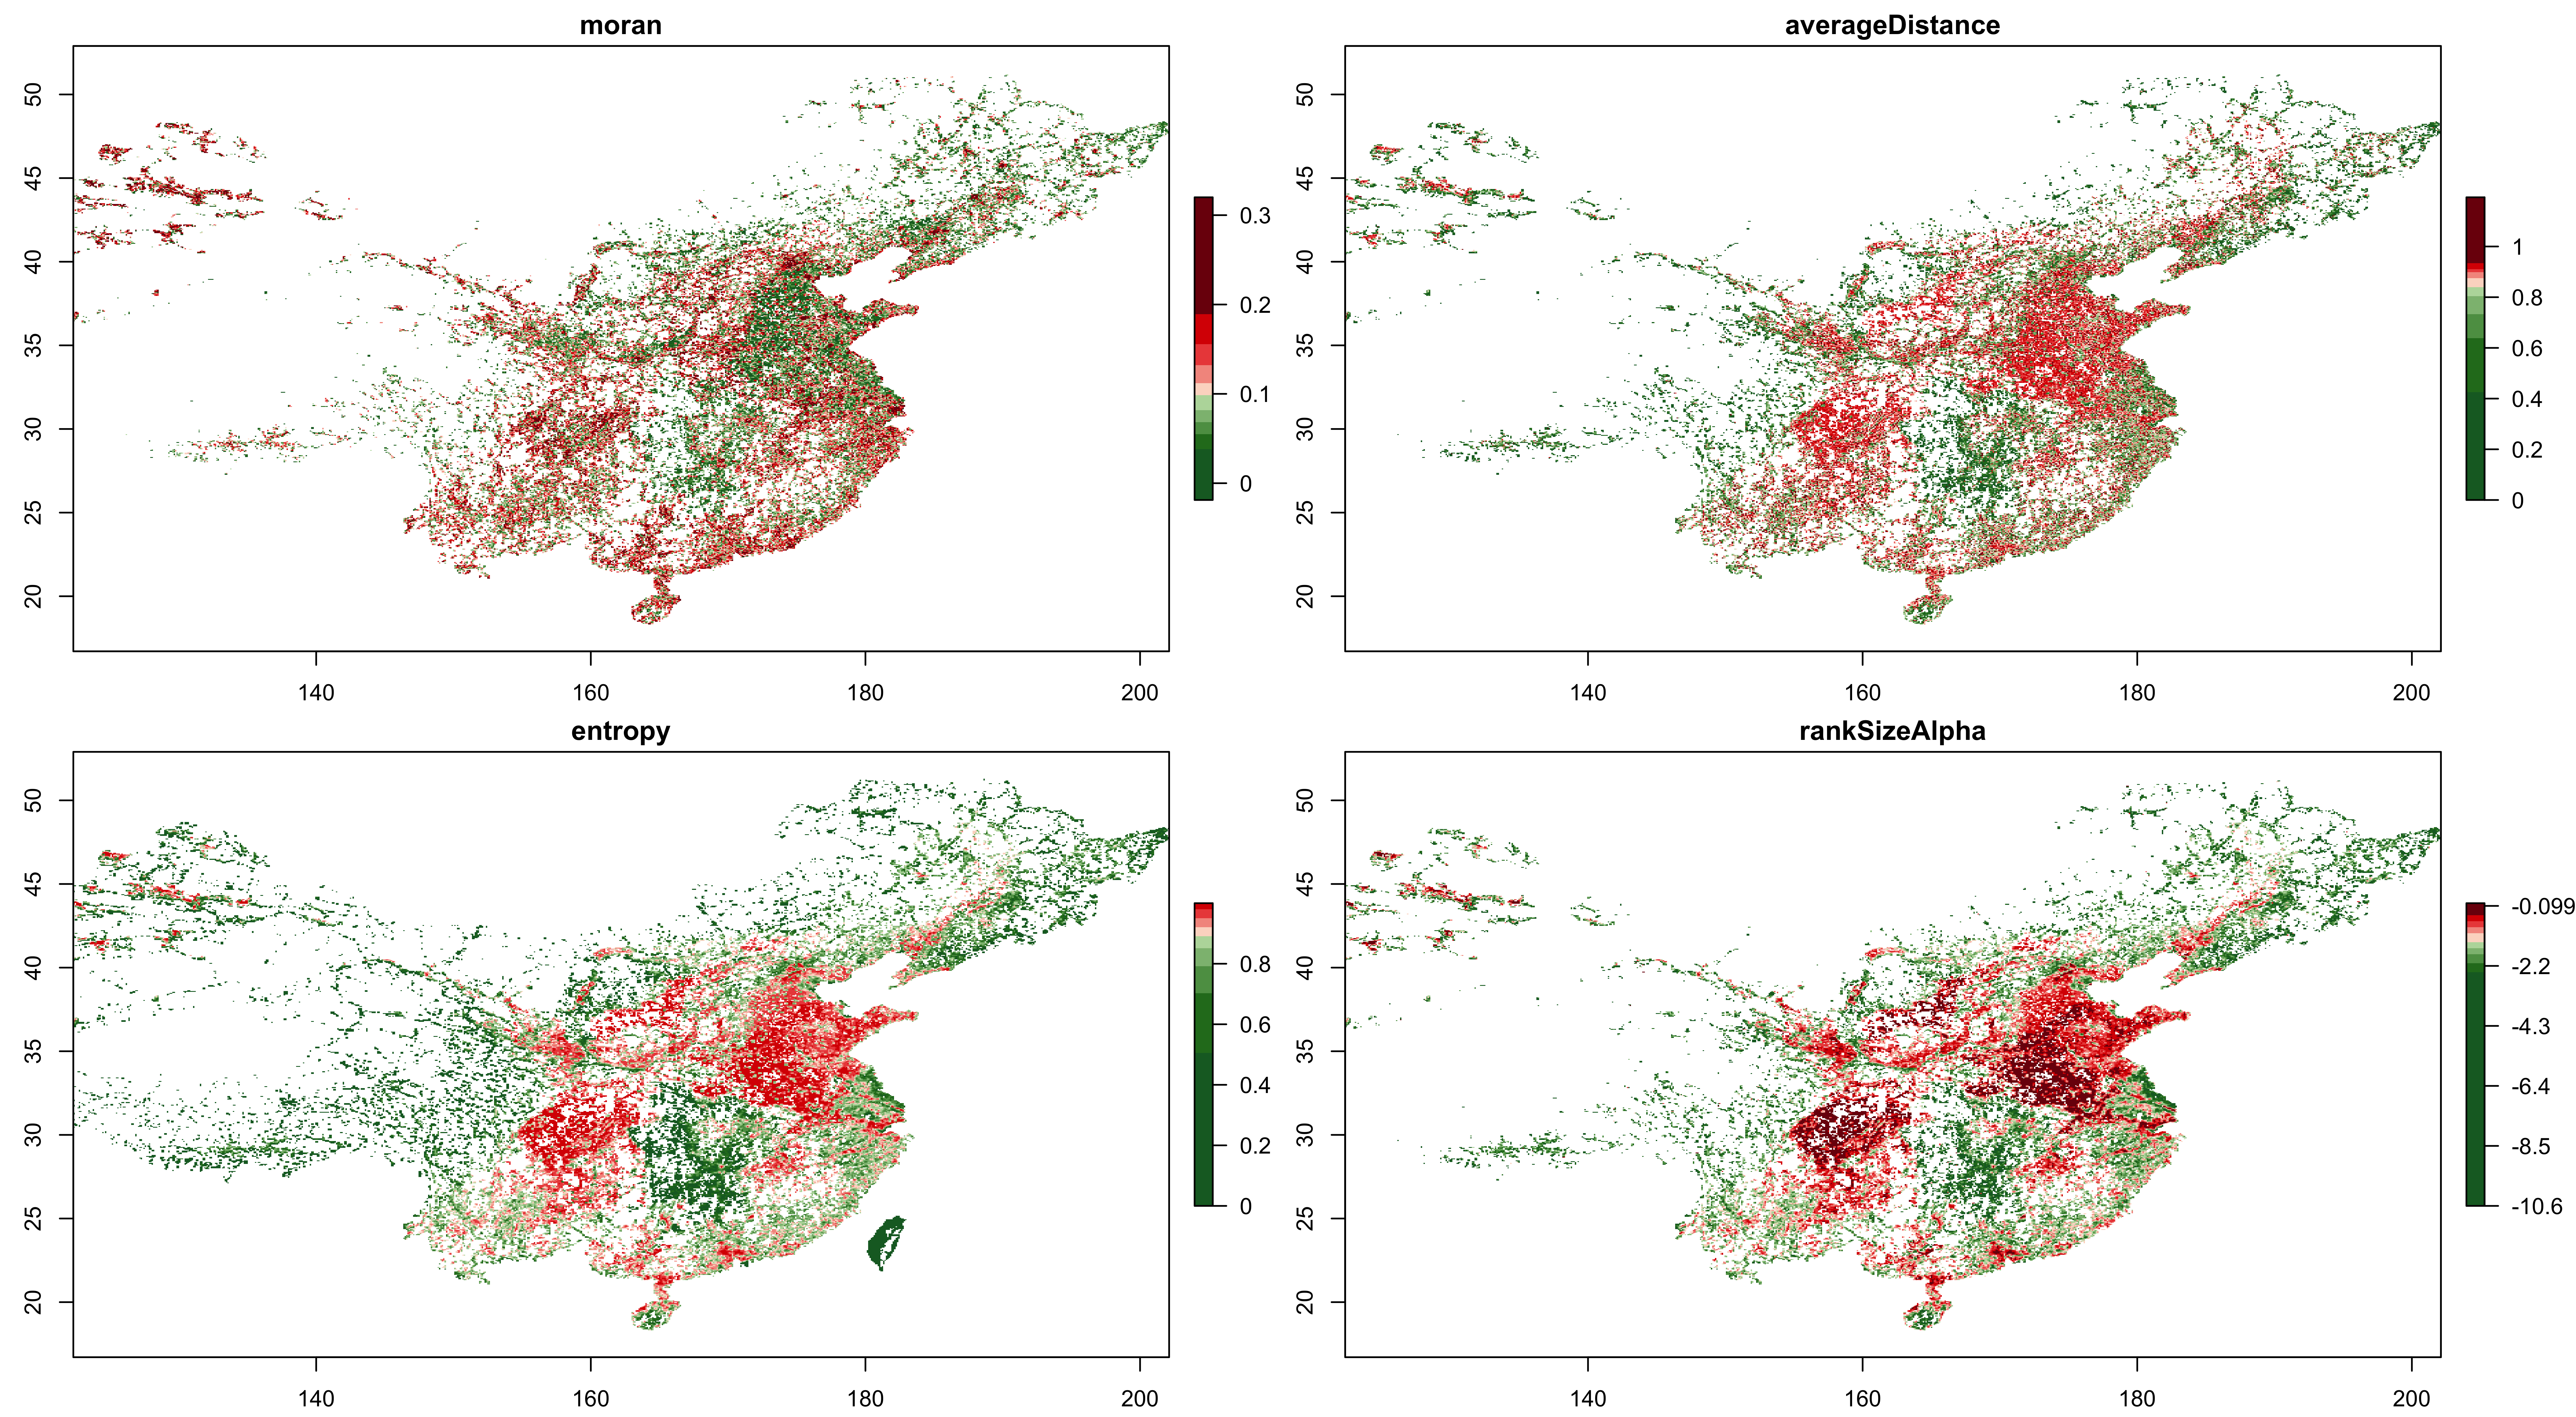
\includegraphics[width=\linewidth]{Figures/StaticCorrelations/CN_indics_morpho}
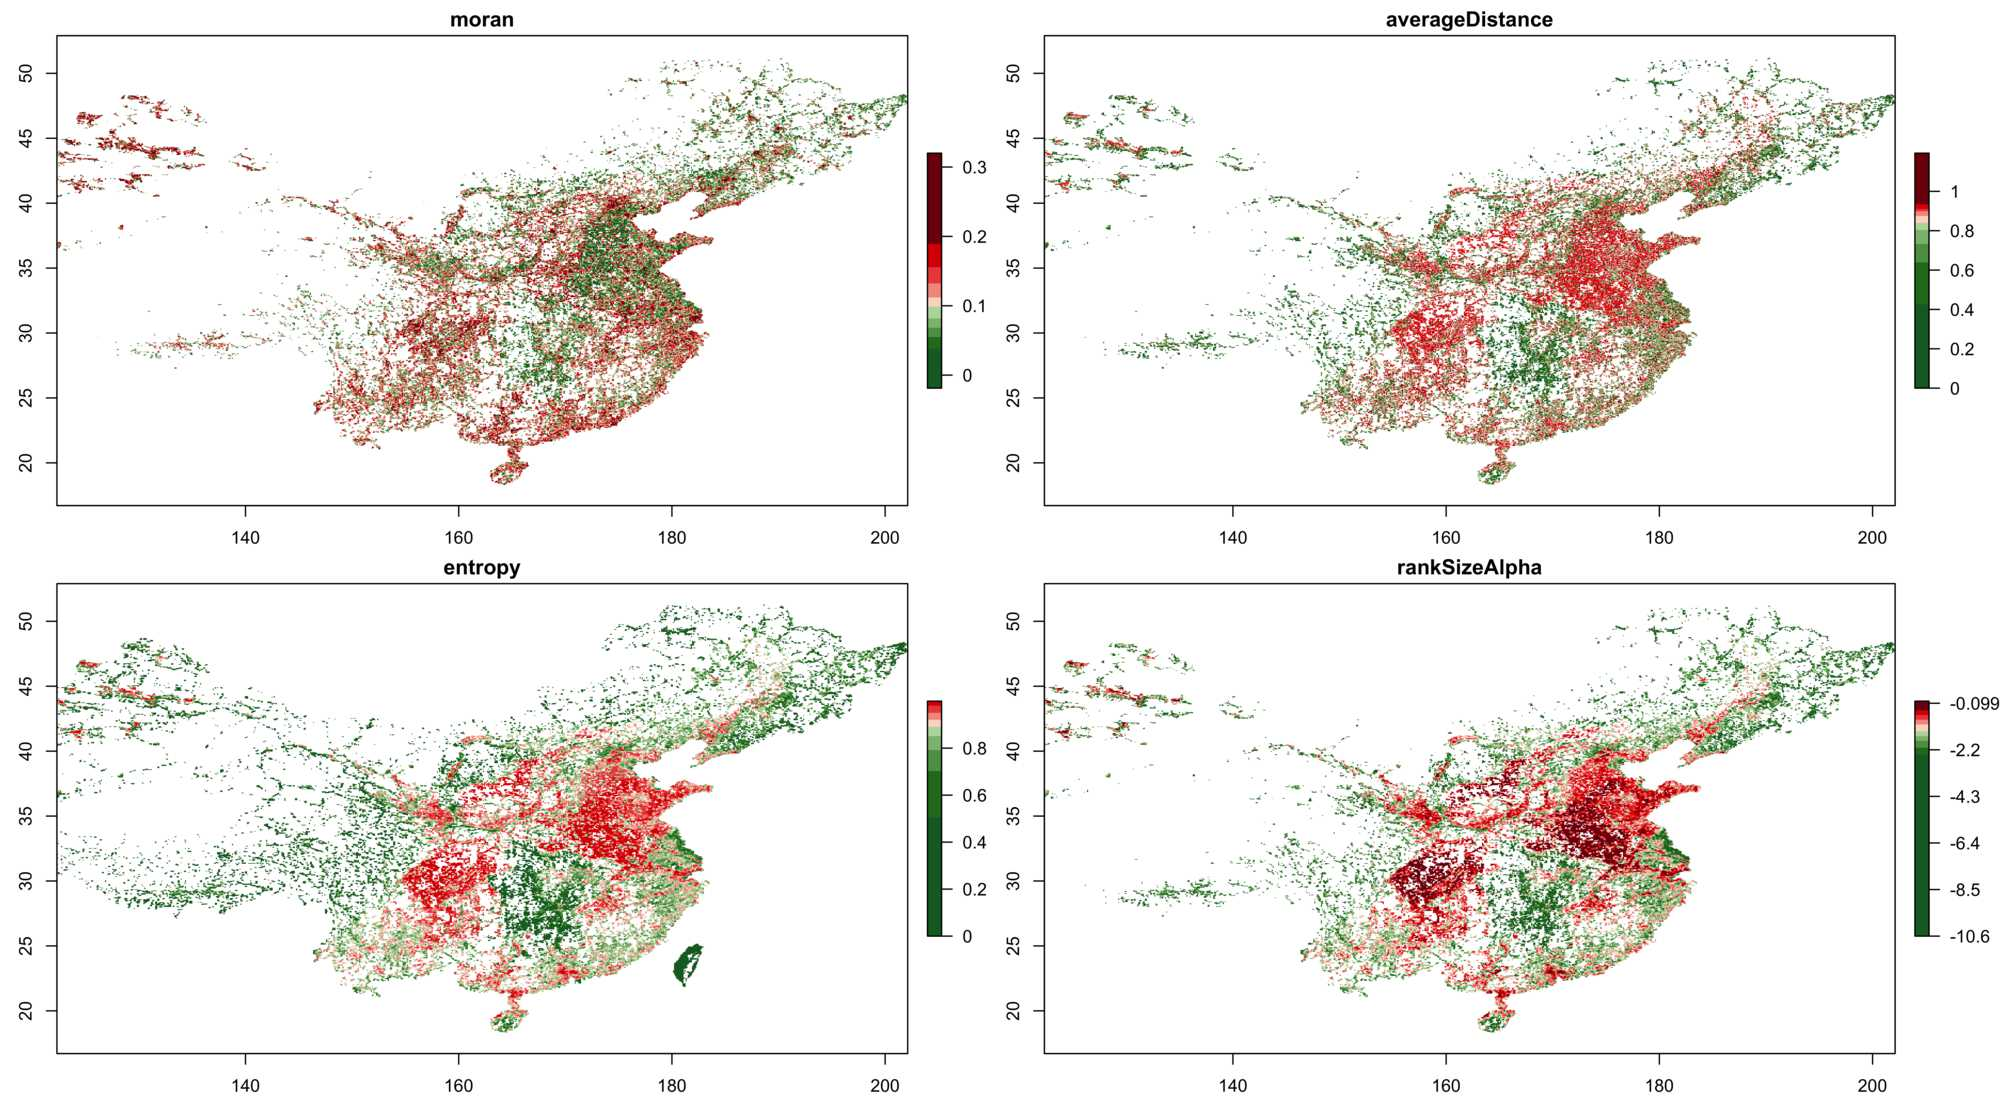
\includegraphics[width=\linewidth]{Figures/Final/A-staticcorrelations-morphocn.jpg}
\appcaption{}{Indicateurs morphologiques pour la Chine.}
\label{fig:app:staticcorrelations:morphocn}
\end{figure}
%%%%%%%%%%%%%%


%%%%%%%%%%%%%%
\begin{figure}
%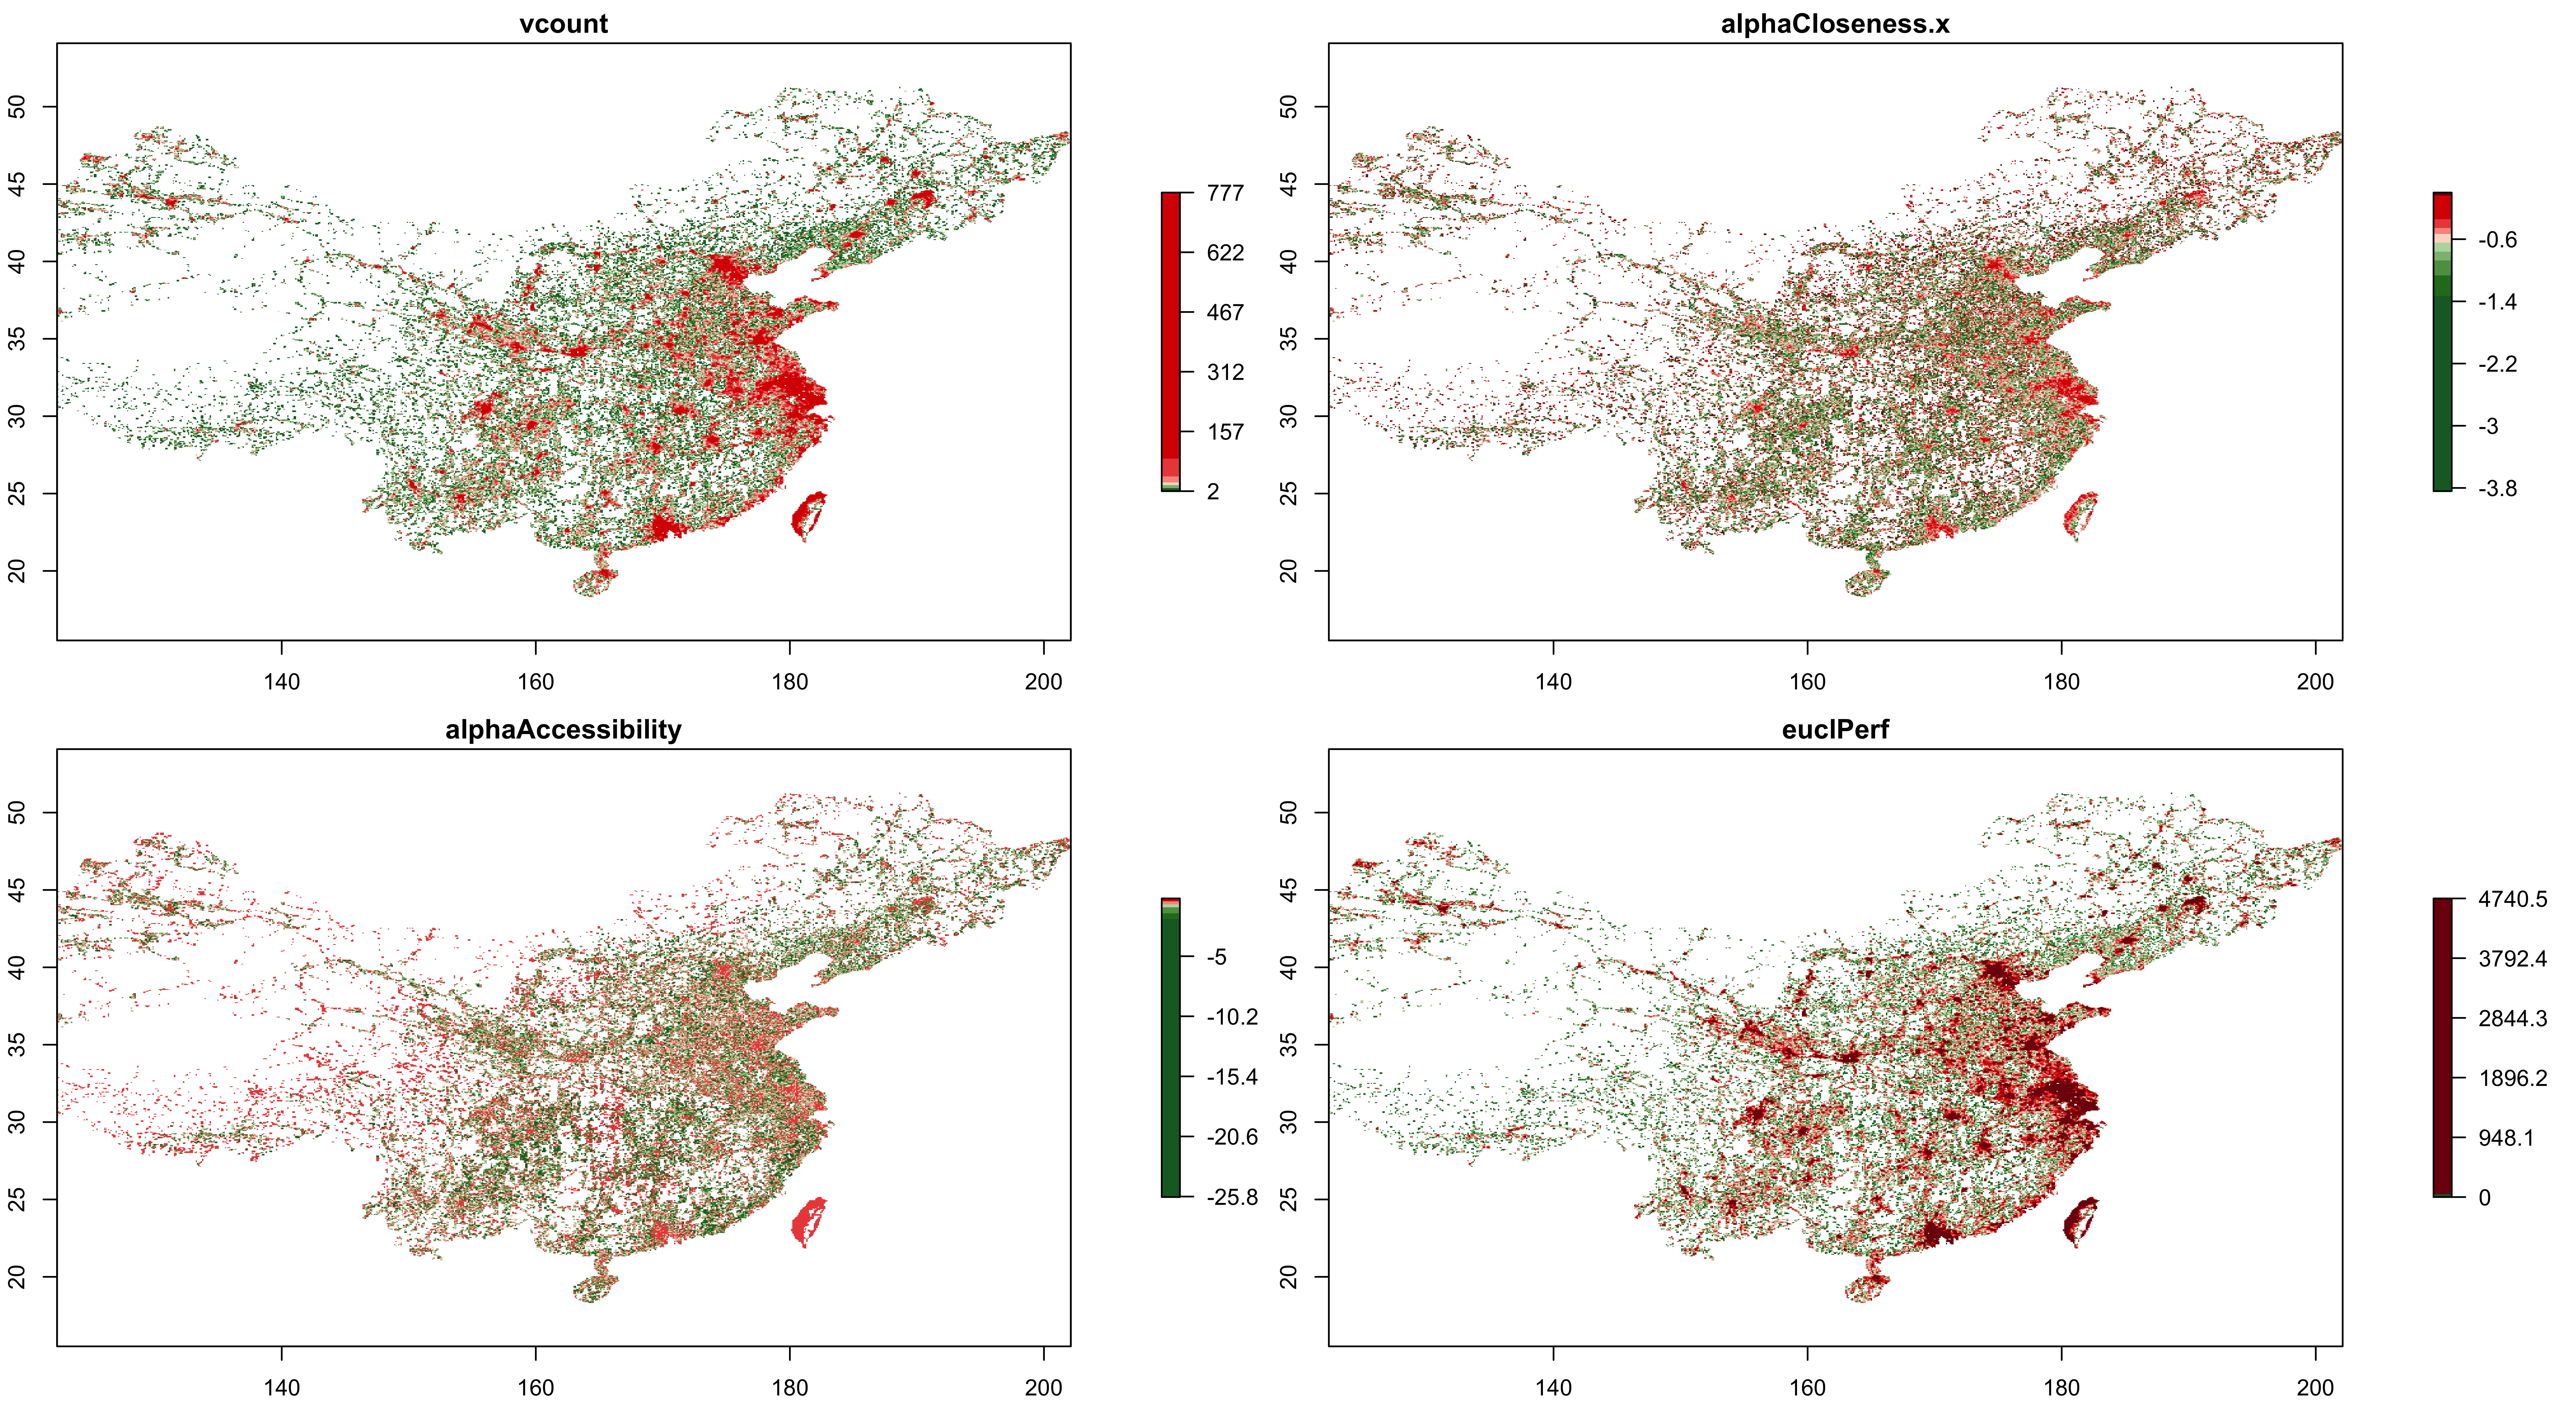
\includegraphics[width=\linewidth]{Figures/StaticCorrelations/CN_indics_network_selected}
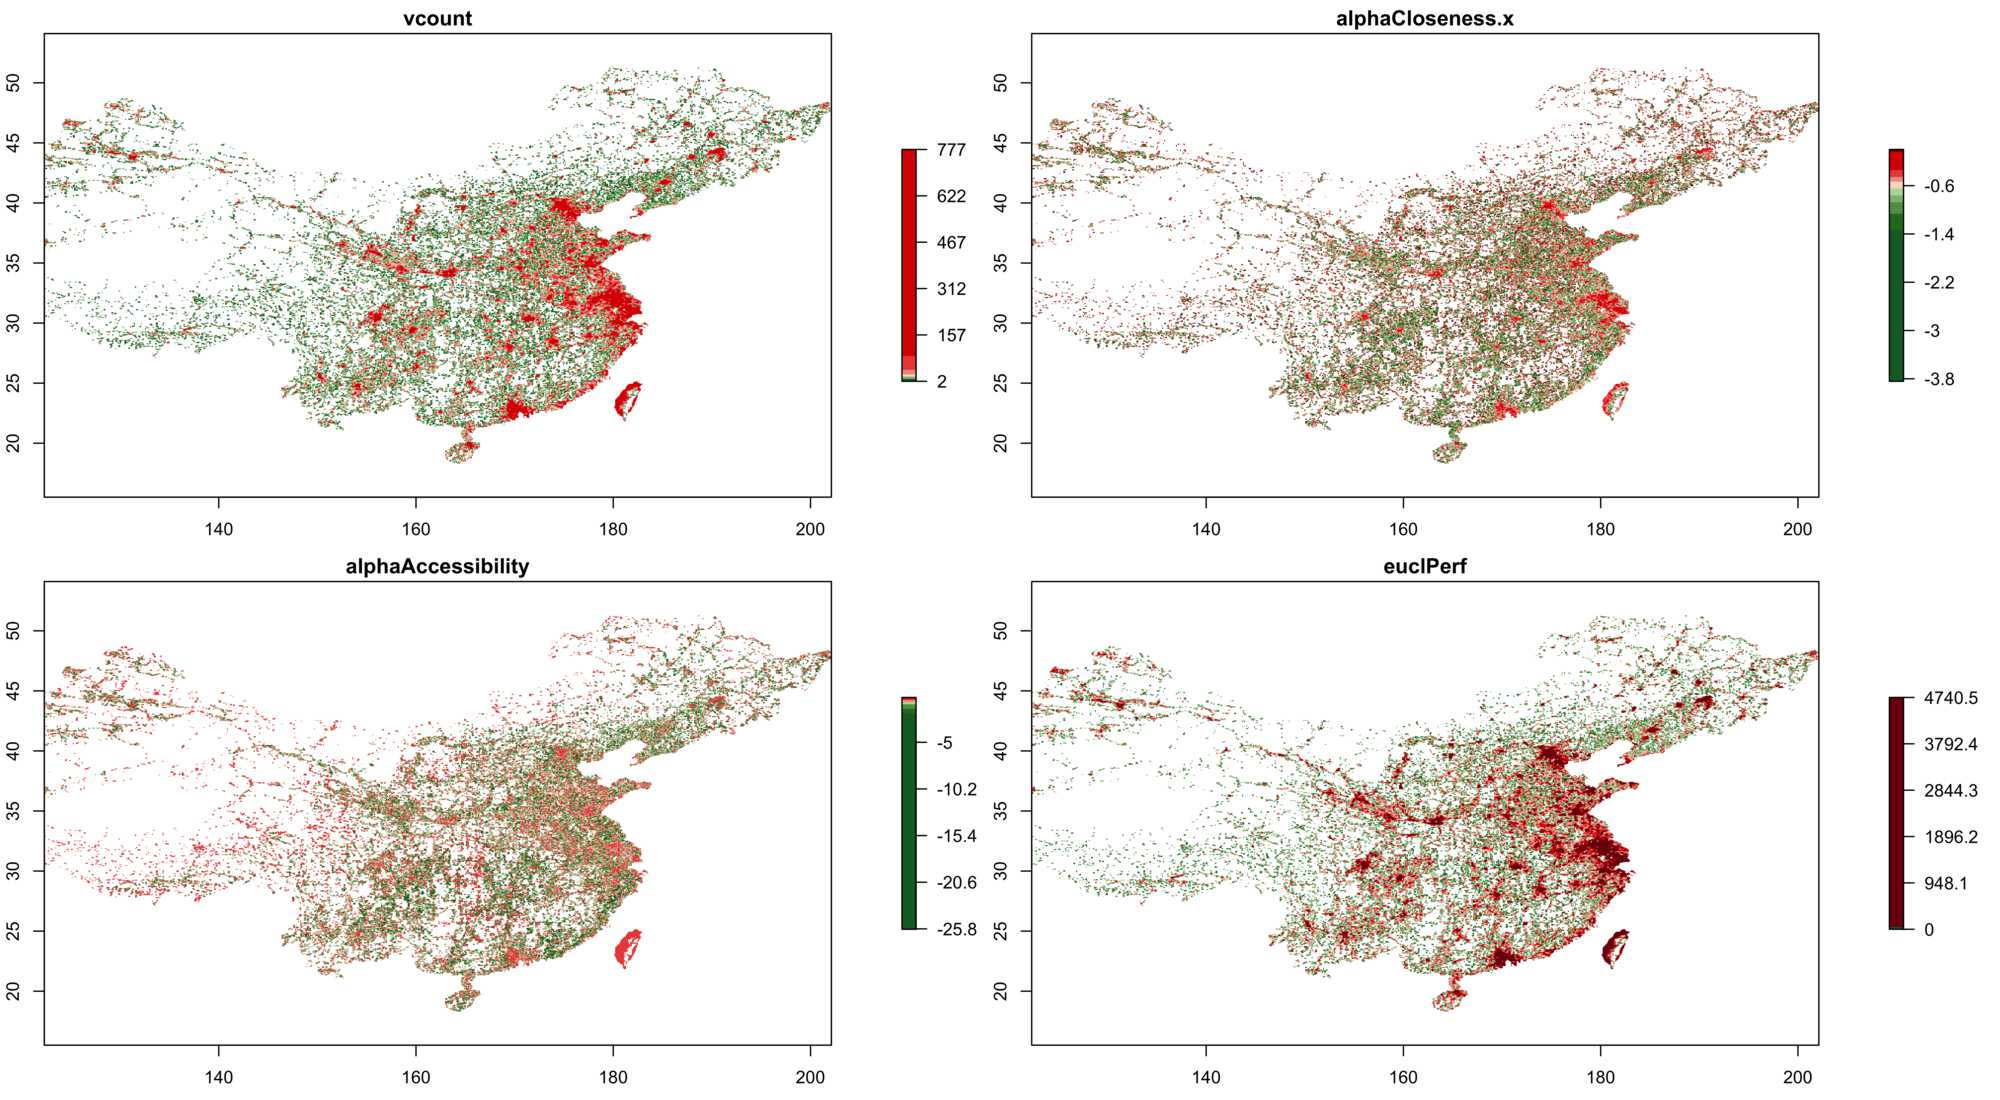
\includegraphics[width=\linewidth]{Figures/Final/A-staticcorrelations-networkcn.jpg}
\appcaption{}{Indicateurs de réseau pour la Chine.}
\label{fig:app:staticcorrelations:networkcn}
\end{figure}
%%%%%%%%%%%%%%



\subsection{Spatial Correlations}{Corrélations Spatiales}

%%%%%%%%%%%%%%
\begin{figure}
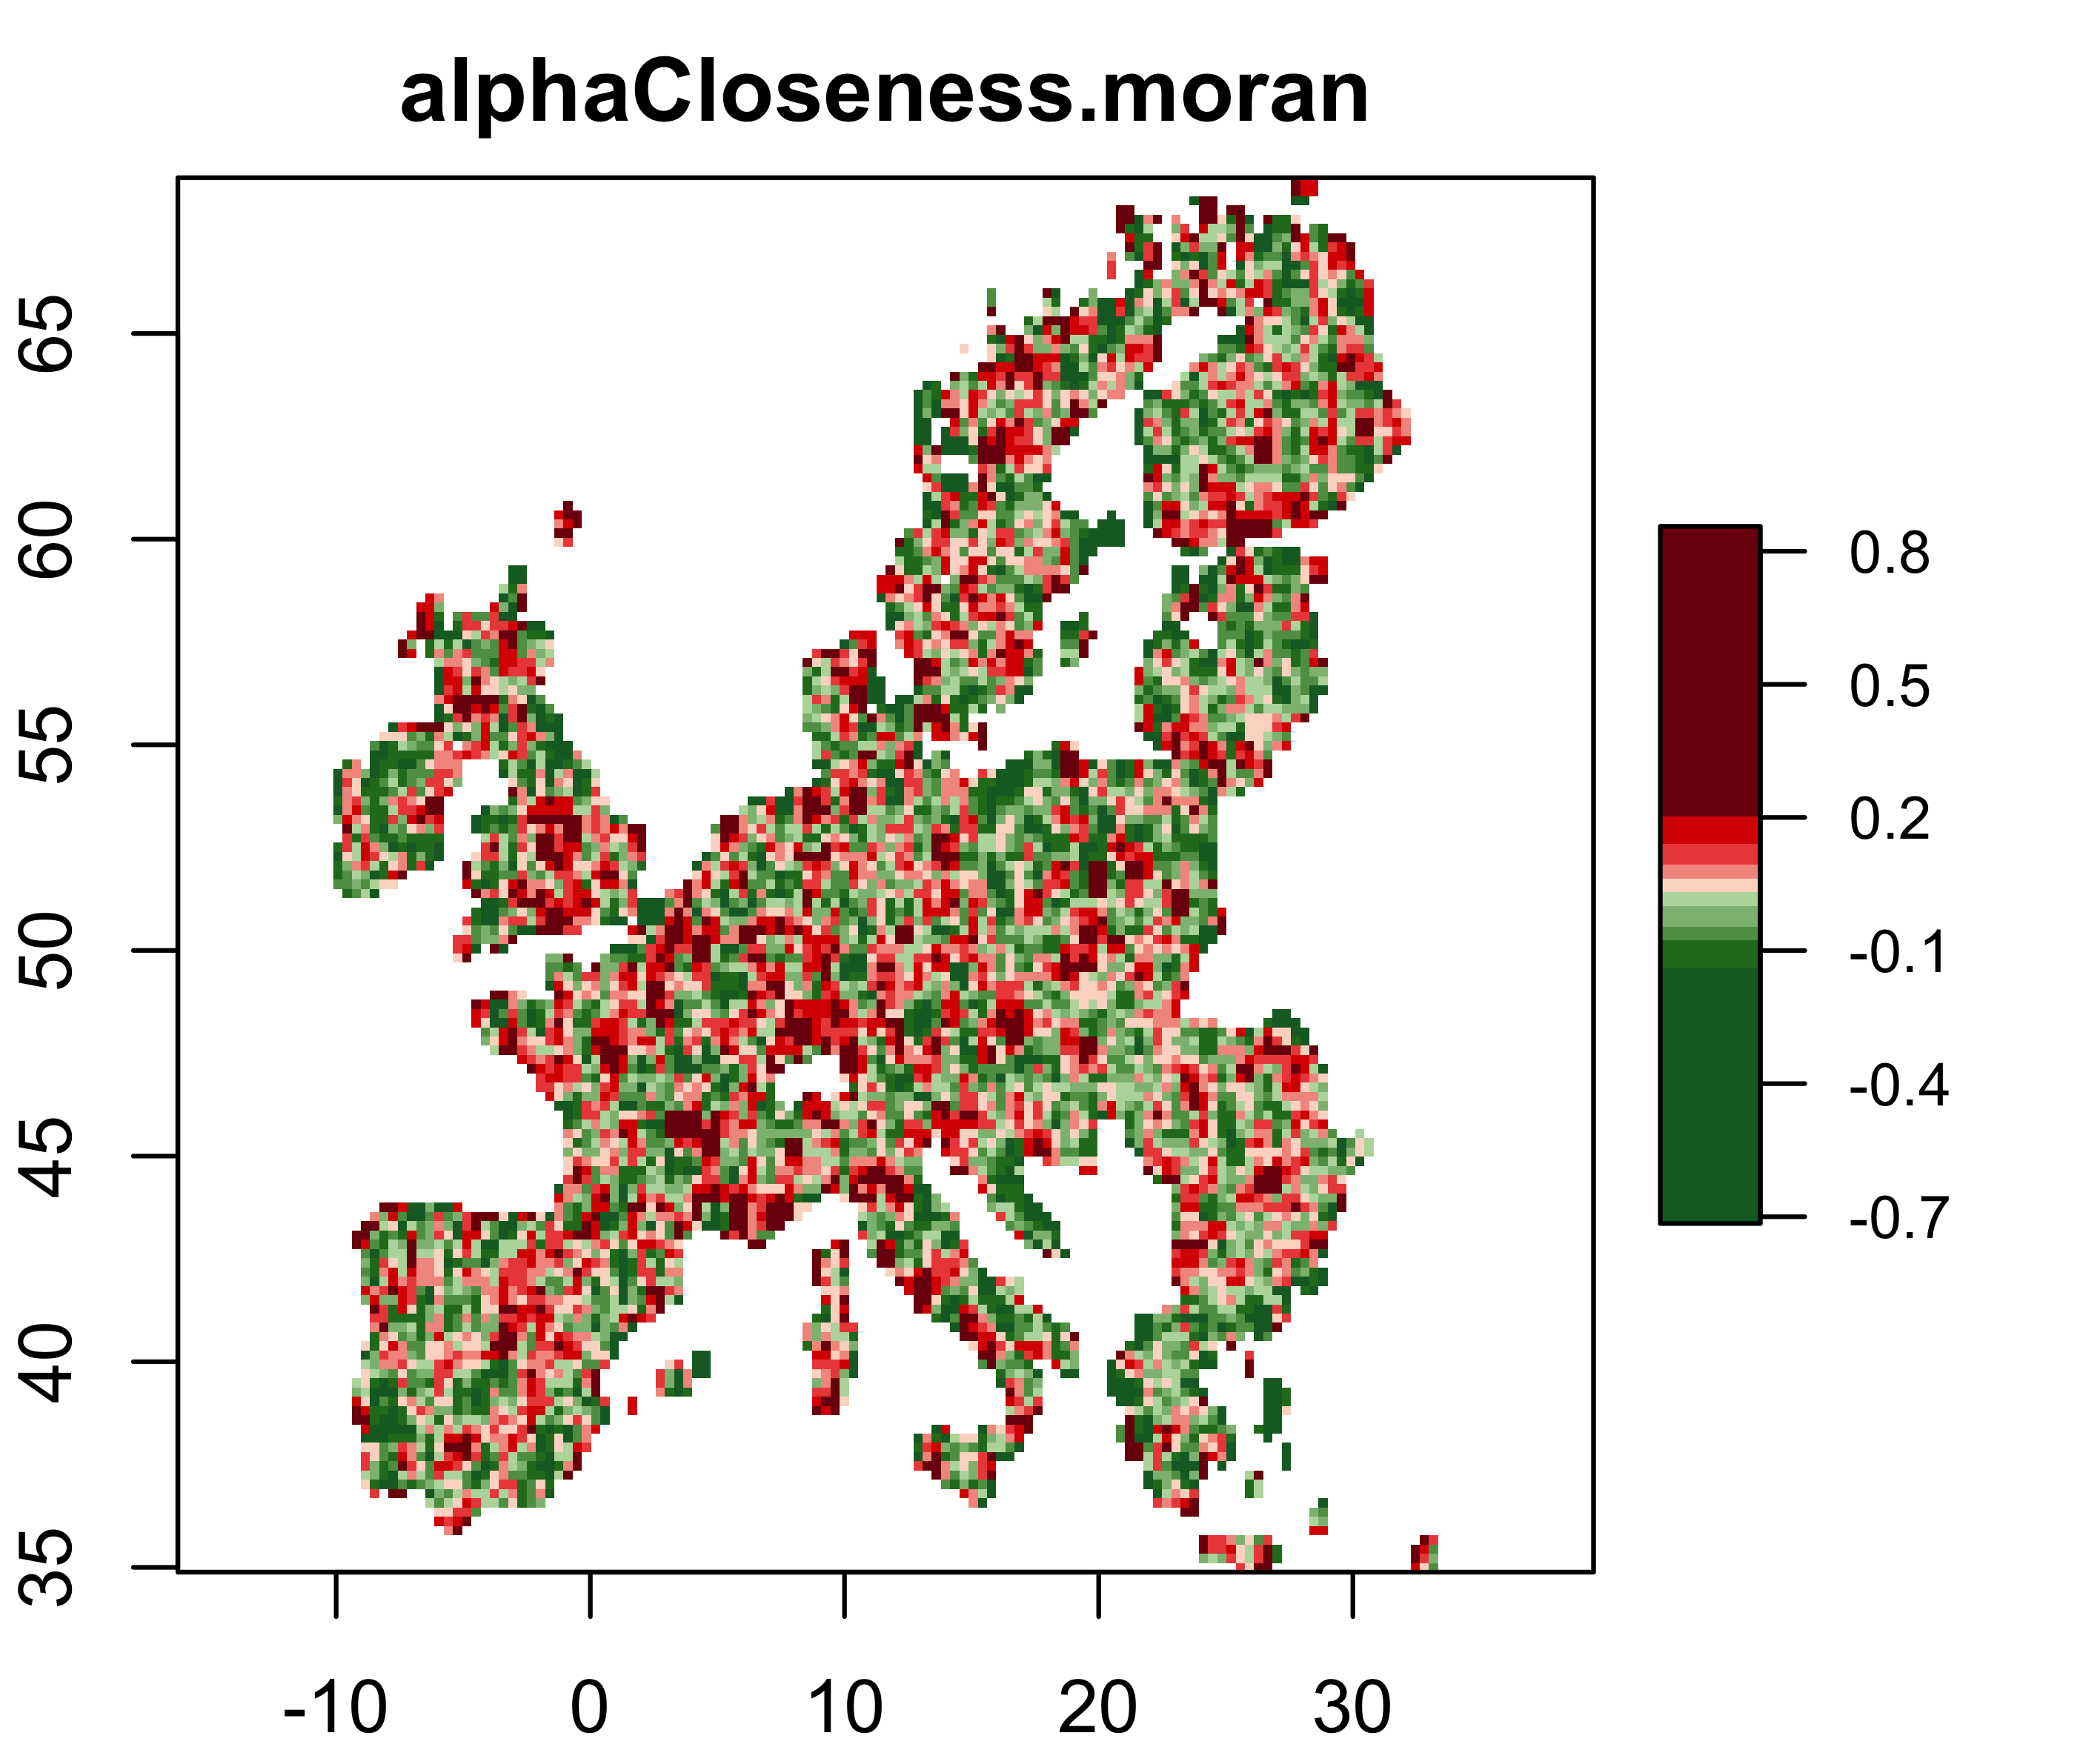
\includegraphics[width=0.48\linewidth]{Figures/StaticCorrelations/EU_corr_alphaCloseness_moran_rhoasize12}
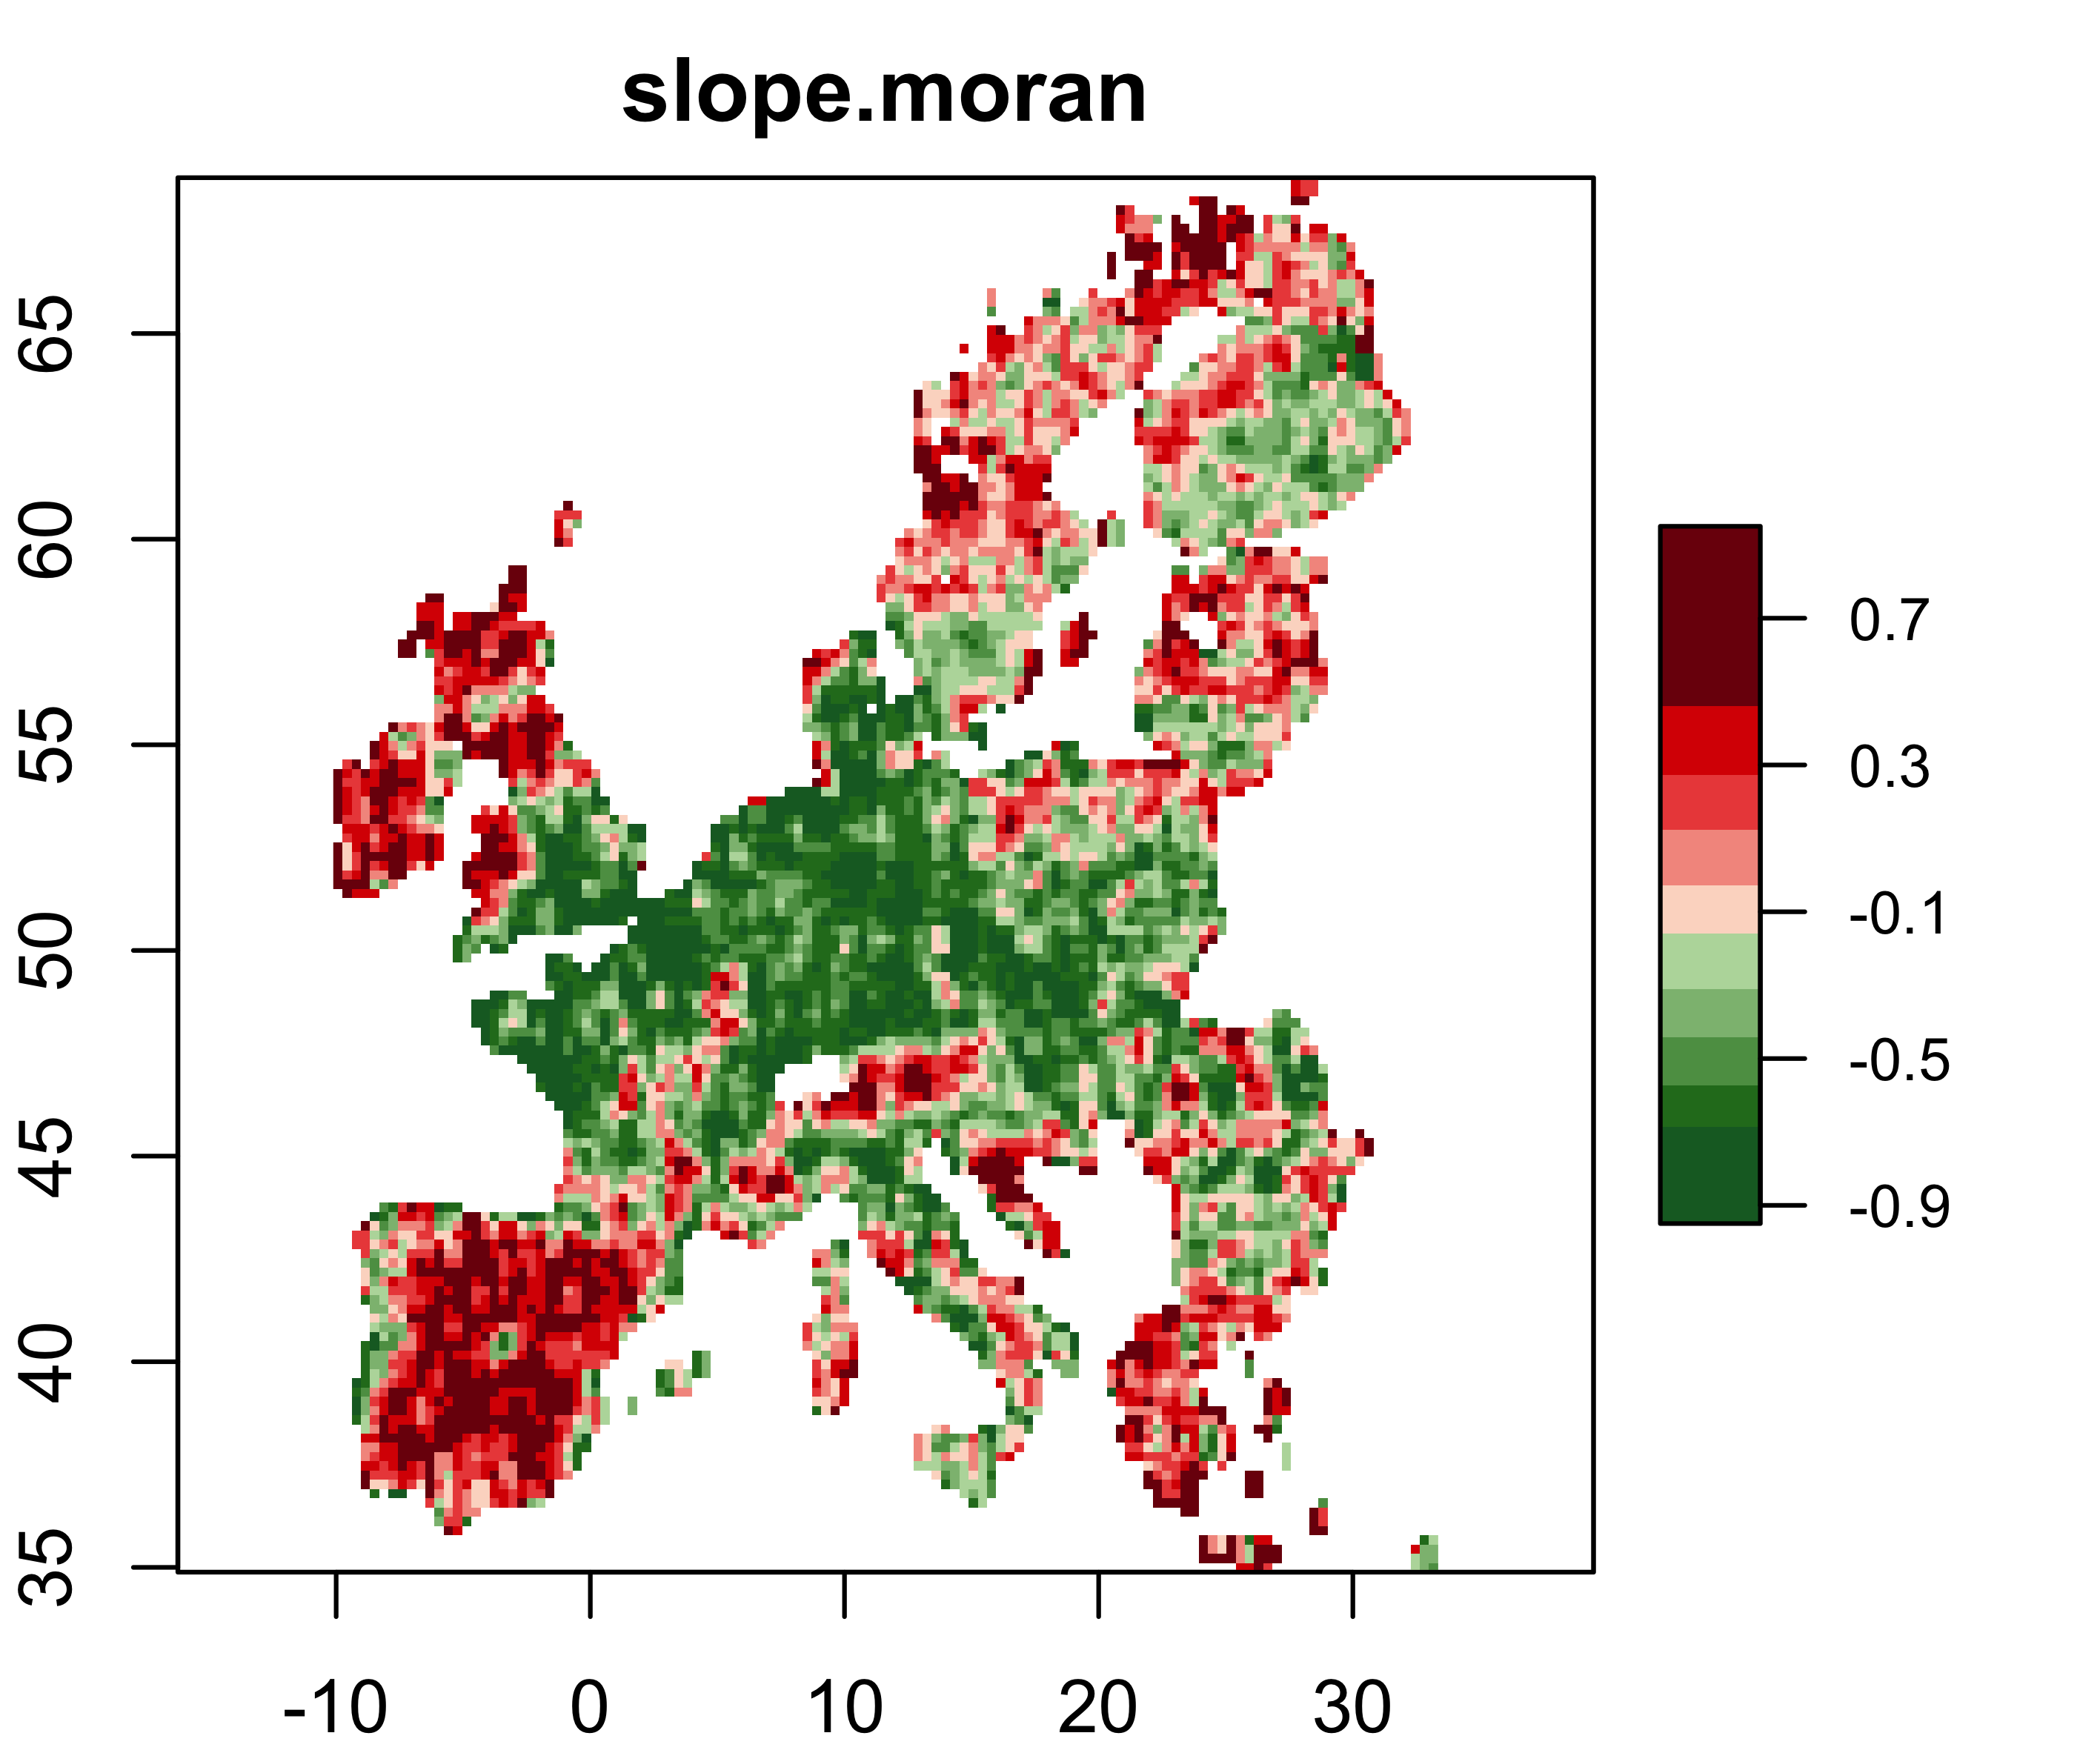
\includegraphics[width=0.48\linewidth]{Figures/StaticCorrelations/EU_corr_slope_moran_rhoasize12}\\
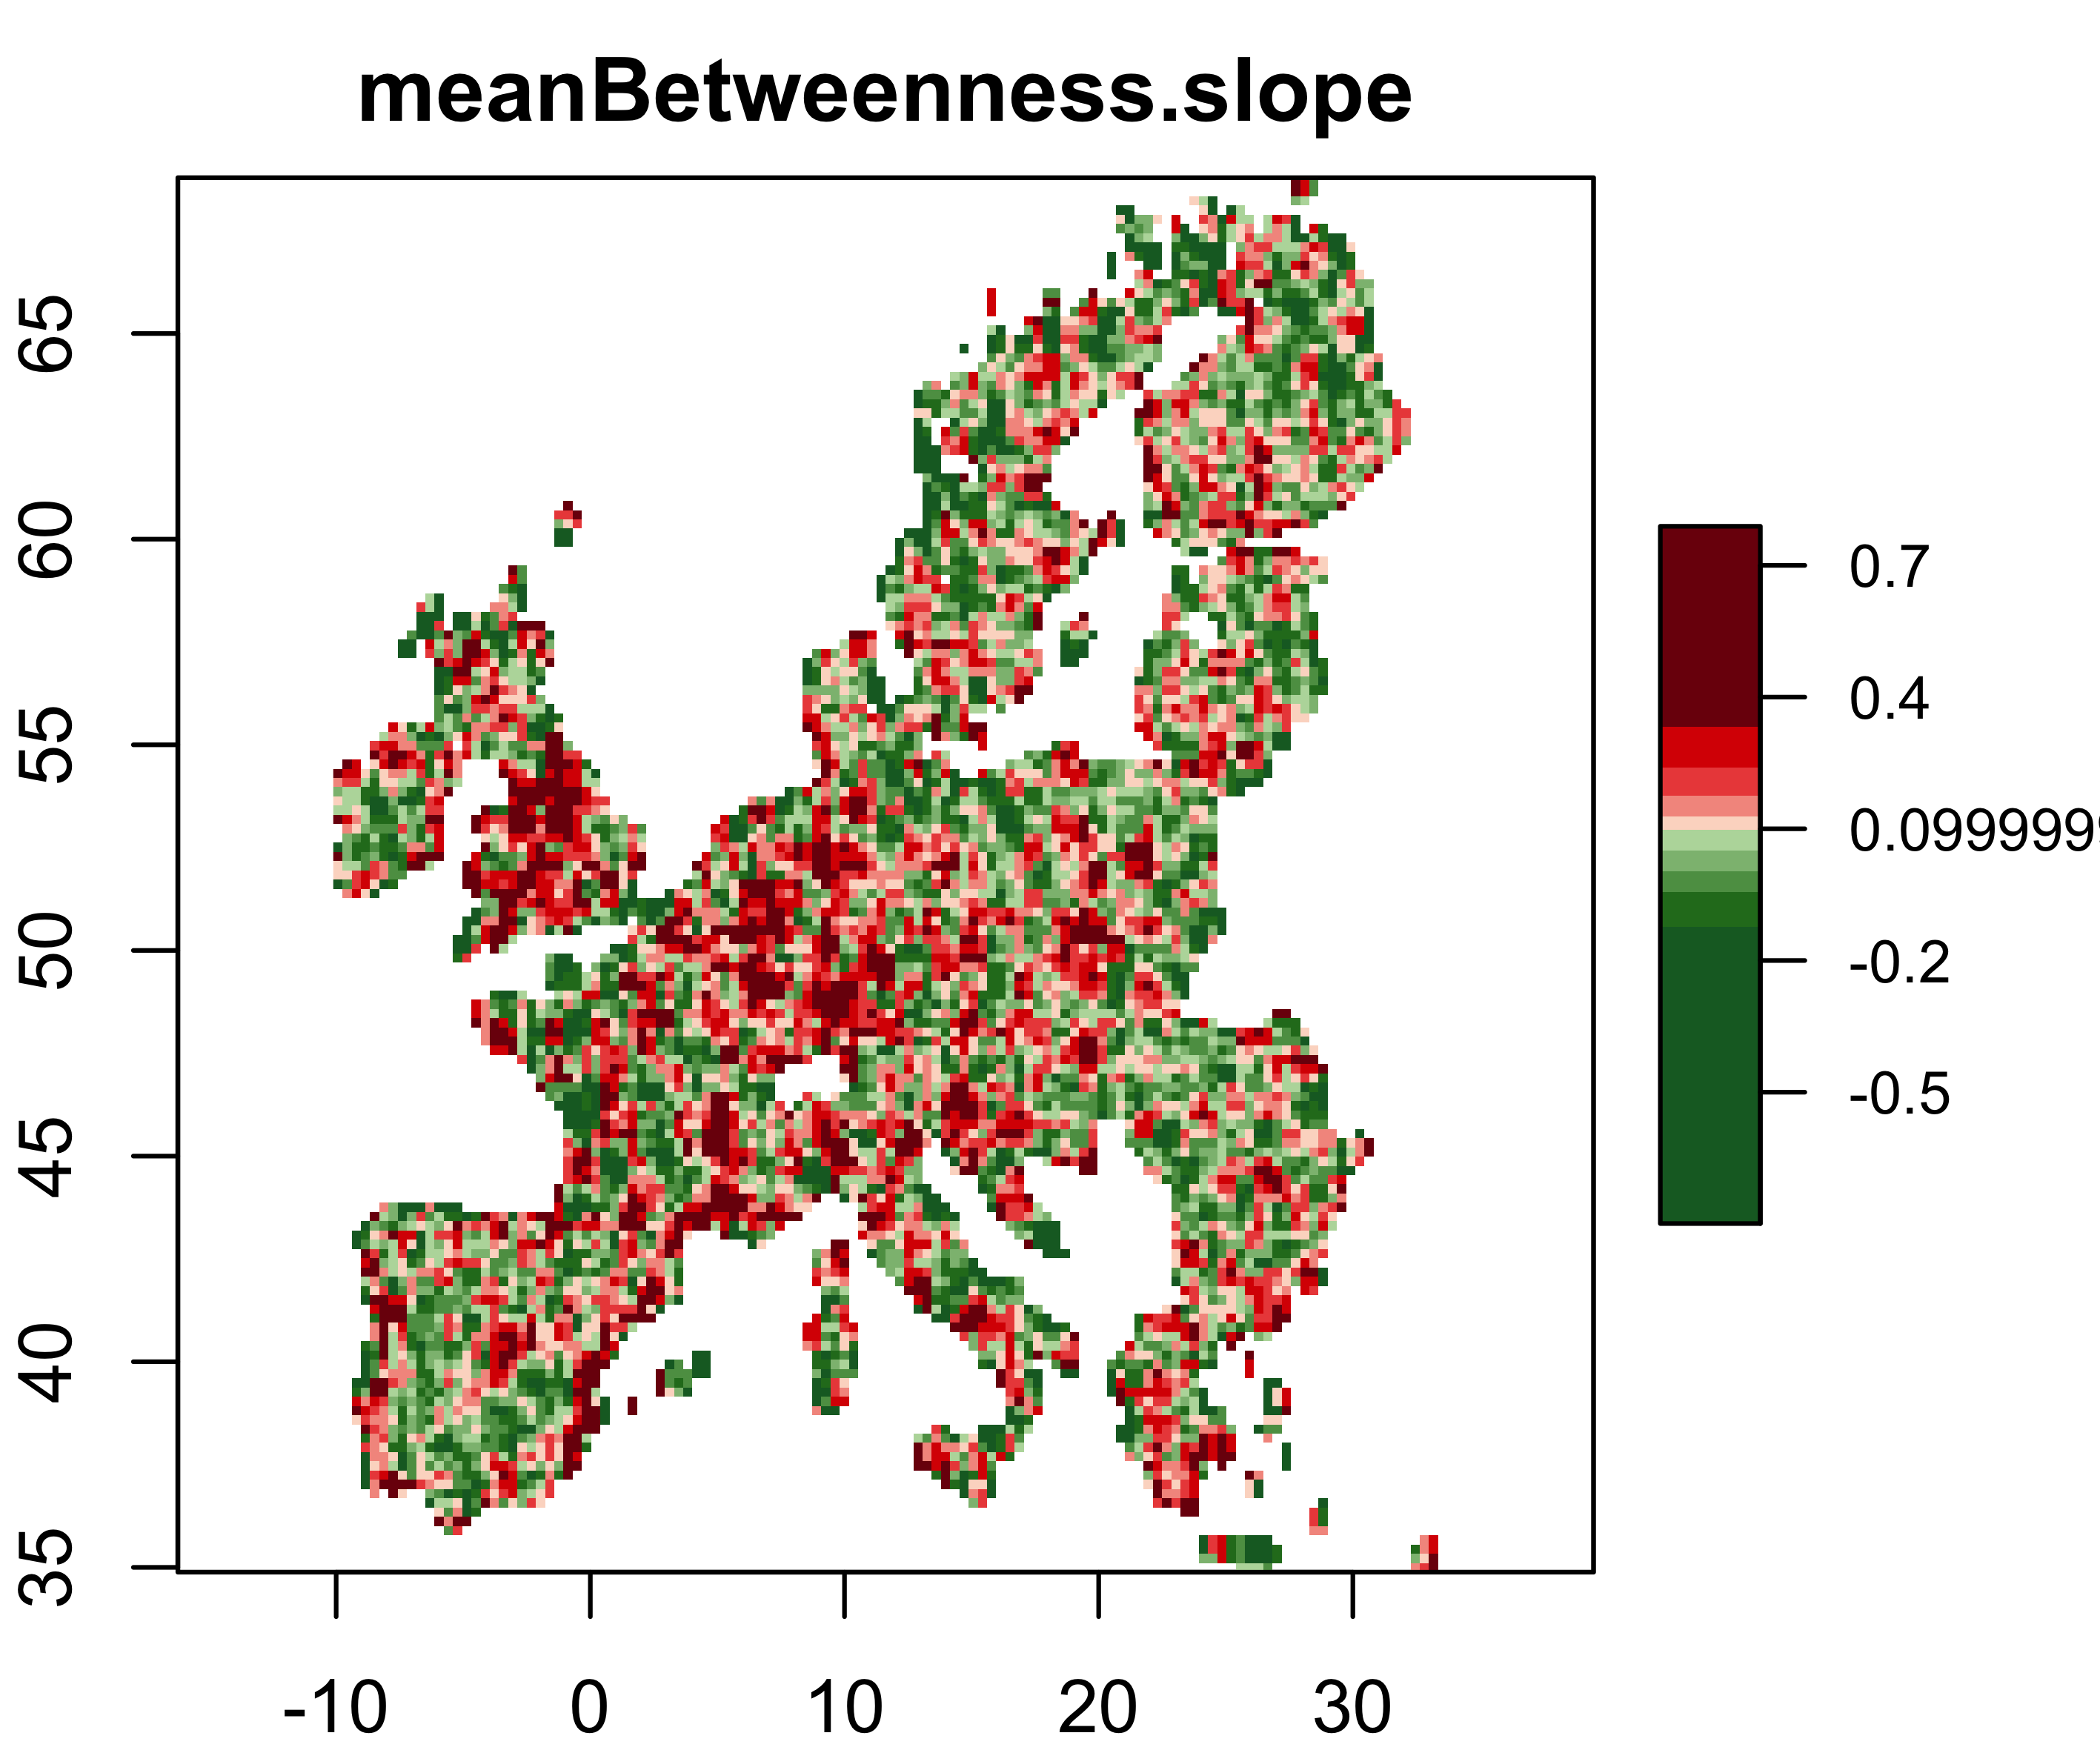
\includegraphics[width=0.48\linewidth]{Figures/StaticCorrelations/EU_corr_meanBetweenness_slope_rhoasize12}
\appcaption{}{Correlations spatiales pour l'Europe.}
\label{fig:app:staticcorrelations:europe_correlations}
\end{figure}
%%%%%%%%%%%%%%






%%%%%%%%%%%%%%
%% -- ON HOLD --

%%%%%%%%%%%%%%
%\begin{figure}
%
%\caption[][]{}{Correlations spatiales pour la Chine.}
%\label{fig:app:staticcorrelations:morphocn}
%\end{figure}
%%%%%%%%%%%%%%




\stars





%----------------------------------------------------------------------------------------

\newpage


%%%%%%%%%%%%%%%%%%%%%%%
\section{Causality regimes}{Régimes de causalité}

\label{app:sec:causalityregimes}






\subsubsection{Context Formalization}{Formalisation}

%\subsubsection{Variables}

%\paragraph{Description}

We assume a dynamic transportation network $n(\vec{x},t)$ within a dynamic territorial landscape $\vec{T}(\vec{x},t)$, which components are to simplify population $p(\vec{x},t)$ and employments $e(\vec{x},t)$. Data is structured the following way :
\begin{itemize}
\item Observation of territorial variables are discretized in space and in time, i.e. the spatial field $\vec{T}$ is summarized by $\mathbf{T} = \left(\vec{T}(\vec{x}_i,t_j^{(T)})\right)_{i,j}$ with $1\leq i \leq N$ and $1\leq j \leq T$. They concretely correspond to census on administrative units (\emph{communes} in our case) at different dates.
\item Network has a continuous spatial position but is represented by the vector of network distances $\mathbf{N}$ \comment{(Florent) vol d'oiseau/distance temps ? second faisable et à privilégier je pense}
\end{itemize}



%\paragraph{Definitions}



\subsubsection{On Accessibility}{Sur l'accessibilité}

% accessibility : need to introduce it ?
%  -> read Weibull

The notion of accessibility has been central to regional science since its introduction and systematization in planning around 1970. 

%\paragraph{Existence of accessibility}

%An elegant axiomatic definition is derived in~\cite{weibull1976axiomatic}. Starting from expected properties of an accessibility function $A$ that associate a value to \emph{attraction} $a$ and distance $d$, defined on the set of discrete spatial configurations $\mathcal{C} = \cup_{n\in \mathbb{N}}{(d_i,a_i)_{1\leq i \leq n}}$. These properties include (among technical others with no thematic meaning) :
%\begin{enumerate}
%\item $A$ is invariant regarding the order of the configuration
%\item $A$ decrease with distance at fixed attraction and increase with attraction at fixed distance
%\item $A$ is invariant when adding null attractions and constant configurations
%\end{enumerate}

%A canonical decomposition of any accessibility function 


As already introduced in the first chapter, we question the notion of accessibility : \textit{Is the notion of accessibility crucial for statistical analysis ?}

\medskip


Weibull has proposed an axiomatic approach to accessibility~\cite{weibull1976axiomatic}, deriving a canonical decomposition for any \emph{attraction-accessibility} function $A(a,d)$, assuming expected thematic axioms among others technical ones that are :
\begin{enumerate}
\item $A$ is invariant regarding the order of the configuration
\item $A$ decrease with distance at fixed attraction and increase with attraction at fixed distance
\item $A$ is invariant when adding null attractions and constant configurations
\end{enumerate}
Then $A$ verifies these if and only if it is of the form

\[
A\left[(a_i,d_i)\right] = T\left(\bigoplus_i z(d_i,a_i)\right)
\]

where $T$ is increasing with null origin, $z$ is a \emph{distance substitution function} (i.e. verifying axiom 2) and $\oplus$ a \emph{standard composition} associating two attractions at zero distance to th corresponding unique one. 

It means that well suited matrices of autocorrelation should capture accessibility in regressions ; \comment{(Florent)pas sur de comprendre, à discuter}
 or it must be captured by non-linear regression on $\mathbf{N}$. It may reveal some kind of intrinsic accessibility that is related to real phenomena (that we expect to fit with calibrated functions of accessibility based on Hedonic models e.g.) Seeing accessibility as a potential field is an equivalent vision : given any stationary dynamic for $n,\vec{T}$, Helmoltz theorem states that it derives from a potential (can be adapted to non-stationary dynamics with a time-varying potential).

%\paragraph{Continuous approach and accessibility potential}

% Paul : Helmoltz-Hodge theorem to infer potential field from speed spatial field ?
%  Q : what are trajectories ? dirac field has no rotational -> continuous approach does not work ?


\subsubsection{Data}{Données}

We will work on a novel dataset provided by \noun{Le Nechet}, that consists in main road infrastructures with their opening dates and train network for network dynamics, and in population and employments of communes at census dates, for Bassin Parisien on the last fifty year. The temporal granularity due to census temporal step may be an obstacle to obtain good dynamical statistics. \comment{(Florent) enfin c'est surtout INSEE, IGN, et Wiki[?] qu'il faut citer (c'est vrai qu'il y a du formatage, mais en tout cas il faut citer les sources de première main)}


\subsubsection{Statistical Tests}{Tests Statistiques}

% Spatial Statistics / causalities ?

The following large set of analysis are to be tested (non exhaustive) :

\comment{(Florent) interprétation ? si O/N}

\begin{itemize}
\item On raw data :
\begin{itemize}
\item Multivariate models
\[\mathcal{L}\left[\mathbf{T},\mathbf{N}\right]\sim \varepsilon\]
\item Autocorrelated univariate models
\[(\mathbf{I} - \Sigma R W) \mathbf{X} \sim \varepsilon\]
\item Autocorrelated multivariate models \[(\mathcal{L}' - \Sigma R W)\left[\mathbf{T}+\mathbf{N}\right] \sim \varepsilon\]
\item Geographically Weighted Regression~\cite{brunsdon1998geographically}
\[
\mathcal{L}\left[\mathcal{G}\left(\mathbf{T},\mathbf{N}\right)\right] \sim \varepsilon
\]
\item Granger causality tests : \cite{xie2009streetcars} use for example Granger causality to link transit with land-use changes.
\end{itemize}
\item On data returns :
\begin{itemize}
\item Autoregressive multivariate models
\[\mathcal{L}\left[(\Delta \mathbf{T}(t_{j'}))_{j'\leq j},(\Delta \mathbf{N}(t_{j'}))_{j'\leq j}\right] \sim \varepsilon\]
\item Autoregressive autocorrelated multivariate models : idem with spatial autocorrelation term.
\item Synthetic Instrumental Variables : static territory and/or network ?
\end{itemize}
\end{itemize}



%\subsubsection{Bivariate linear models}

%\subsubsection{Autocorrelated univariate models}

%\subsubsection{Autocorrelated multivariate models}

%\subsubsection{Granger causality tests}

%\cite{xie2009streetcars} use Granger causality to link transit with land-use changes.

%\subsubsection{Autoregressive multivariate models}

%\subsubsection{Autoregressive autocorrelated multivariate models}



%\subsection{Expected results}

%We expect from these analyses to test at these spatial and temporal scales, and on a particular metropolitan case study, the assumption on network necessity for the territorial system of functional job commutings.





\stars


%----------------------------------------------------------------------------------------


\newpage

%%%%%%%%%%%%%%%%%%%%%%%
\section{Network Effects}{Effets de réseau}

\label{app:sec:interactiongibrat}








%We can develop the difference in information between two computational models, given by the difference of Kullback-Leibler information, 

%\[
%\Delta D_{KL} \left(M^{(1)}|M^{(2)}\right) = \Delta D_{KL} \left(S^{(1)}|S^{(2)}\right) + \left[ \Delta D_{KL} \left(S^{(2)}|M^{(1)}\right) + \Delta D_{KL} \left(S^{(1)}|M^{(2)}\right) \right]
%\]
 

%Under certain assumptions, the order of magnitude of second term appears to be negligible. More precisely, with $s^{(k)} = S^{(k)} - M^{(k)}$ and $f$ the probability density of reality the models try to approach, we have

%\[
%\begin{split}
%\Delta D_{KL} \left(S^{(k)}|M^{(k')}\right) & = \norm{\int f \cdot\log{\left(\frac{S^{(k)}}{M^{(k')}}\right)}} = \norm{\int f\cdot \log{\left(1 + \frac{s^{(k)}}{M^{(k')}}\right)}}\\
%& \simeq \norm{\int f \cdot \frac{s^{(k)}}{M^{(k')}}} \leq \frac{\sqrt{s_k}}{\norm{M^{(k')}}} \int f \leq 
%\end{split}
%\]
%



%%%%%%%%%%%%%%%%%%%%%%%%%%%
%\subsection*{Methodological implications}
%  - reflexions on iterative calibration, here ?
% no
%  - multimodeling ; back to the simple
% - bayesian iterative formulation ? (mcmc)
% - how does formulation influence ? equivalence in certain cases between stoch-cov and interdependent expectancies ? : under which conditions we can impose a covariance structure that produces interdependencies between expectancies ? seems to be a very broader question, need to do some thinking on that.











